\section{Case Studies}
\subsection{Multiple Host Headers}
\textbf{Case 1}
\vspace{1ex}
\begin{spacing}{0.8}
	\begin{tcolorbox}
	
		\textbf{RFC 2616}
		Multiple message-header fields with the same \texttt{field-name} MAY be present in a message {\color{red}{ if and only if (隐晦地说明Multiple Host是不允许的)}} the entire \texttt{field-value} for that header field is defined as a comma-separated list. It MUST be possible to combine the multiple header fields into one ``\texttt{field-name: field-value}'' pair, without changing the semantics of the message, by appending each subsequent field-value to the first, each separated by a comma. 
	\end{tcolorbox}
\end{spacing} 

\vspace{1ex}

\begin{spacing}{0.8}
		\begin{tcolorbox}
		\textbf{RFC 7230} 
		A sender {\color{red}{MUST NOT}} generate multiple header fields with the same field name in a message unless either the entire field is defined  as a comma-separated list ...
	
		A recipient MAY combine multiple header fields with the same field name into one ``\texttt{field-name: field-value}'' pair, without changing the semantics of the message, by appending each subsequent field value to the combined field value in order, separated by a comma. 
	\end{tcolorbox}
\end{spacing}

\vspace{1ex}

\begin{spacing}{0.8}
	\begin{tcolorbox}
		\textbf{RFC 7230}
		A server {\color{red}{MUST respond with a 400 (Bad Request)}} status code to any HTTP/1.1 request message that lacks a \texttt{Host} header field and to any request message that {\color{red}{contains more than one \texttt{Host} header field}} or a \texttt{Host} header field with an invalid field-value. (Page 44)
	\end{tcolorbox}
\end{spacing}

\vspace{2ex}


\begin{figure*}[!htbp]
	\centering
	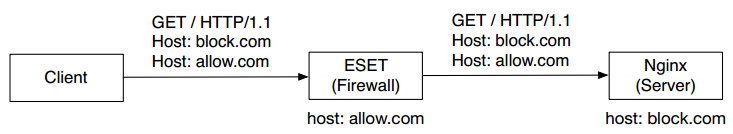
\includegraphics[width=1.0\textwidth]{Preference_Multi-Host.jpg}
	\caption{Preference of multiple \texttt{Host} headers.}
	\label{fig:preference_multi-Host}
\end{figure*}

首先,在同一个Request中出现多个\texttt{Host}本来就是非法的,而ESET和Nginx都允许这种情况出现。其次,面对多个\texttt{Host},二者选择的方式不一样,见下表:

\begin{tabular}{|c|c|c|}
	\hline 
	\textbf{实现(工具)} & \textbf{多\texttt{Host}的处理} & \textbf{对Request的转发}  \\  
	\hline 
	ESET & 取\textbf{最后一个}\texttt{Host} & 原样转发 \\ 
	\hline 
	Nginx & 取\textbf{第一个}\texttt{Host} & \\
	\hline
	\hline
	RFC 2616 & Reject & \\
	\hline
	RFC 7230 & Reject & 见下方描述\\
	\hline
\end{tabular} 

\begin{spacing}{0.8}
	\begin{tcolorbox}
		\textbf{RFC 7230 有关如何解析Host和转发Request}
		 
		When a proxy receives a request with an absolute-form of request-target, the proxy MUST ignore the received \texttt{Host} header field (if any) and instead replace it with the host information of the
		request-target (Absolute-URI中的Host信息优先). A proxy that forwards such a request {\color{red}{MUST generate a new Host field-value based on the received request-target}} rather than forward the received \texttt{Host} field-value. (Page 44)
	\end{tcolorbox}
\end{spacing}

\vspace{2ex}

\textbf{Case 2}

\begin{figure*}[tbph!]
	\centering
	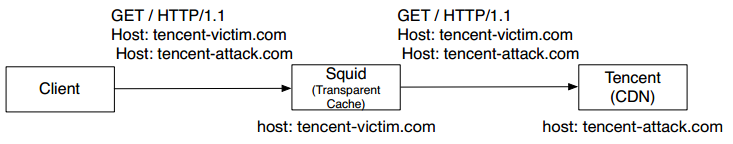
\includegraphics[width=1.0\linewidth]{images/Multi-Host_Preceding_Space}
	\caption{Multiple \texttt{Host} headers with preceding space}
	\label{fig:multi-hostprecedingspace}
\end{figure*}


